\section{Interactive Visualization Design Environment}
\label{sec:environment}
In this section, we will describe our web-based visualization design environment, VisComposer.

\subsection{The Interface}
The interface (Figure~\ref{fg:interface}) contains four main views corresponding to four modules of the visualization composition model. All widgets and views are designed to be collapsible so that more
screen space can be preserved for the main view.

The \textbf{resource} view~(Figure~\ref{fg:interface} (a)) shows the resources being used in designing visualizations. The view contains four main components that list the names, structures and properties of data and the data primitives, composition operators and visual forms. Detailed information of selected items (e.g., the input dataset) can be further explored using additional popup windows. Our system supports the loading and composition of multiple datasets and visual forms.

The \textbf{visualization} view (Figure~\ref{fg:interface} (b)) is the container of the visualization being designed.  It is updated whenever a modification is made during the design process. To enable quick design iterations, the view is synchronized with the creation of the scenegraph.  A proxy geometry or graphical glyph is shown if a node or link of the underlying scenegraph has not been bound, or if a primitive has not been mapped to a visual propertiy. Interactive specification and manipulation of the graphical primitives or forms in the view is allowed.

The \textbf{scenegraph} view (Figure~\ref{fg:interface} (c)) shows the scenegraph structure of the visualization and enables many user interactions that represent the abstract and interact operations defined in Section 5.1. The user can create nodes, links and compose the visualization within this view. The tree shows the basic information of each node and link, such as the type of primitives, the underlying data selectors and the composition operators. The user can edit nodes and links interactively or load from stored forms as a prototype template.

The \textbf{transformation} view is the workbench for performing the bind, map and abstract operations. A suite of textual and configuration panels (Figure~\ref{fg:interface} (d)) are provided for user modulations. The user can craft transformations by editing ones provided by the system or write a visualization shader.

\begin{figure*}
  \centering
  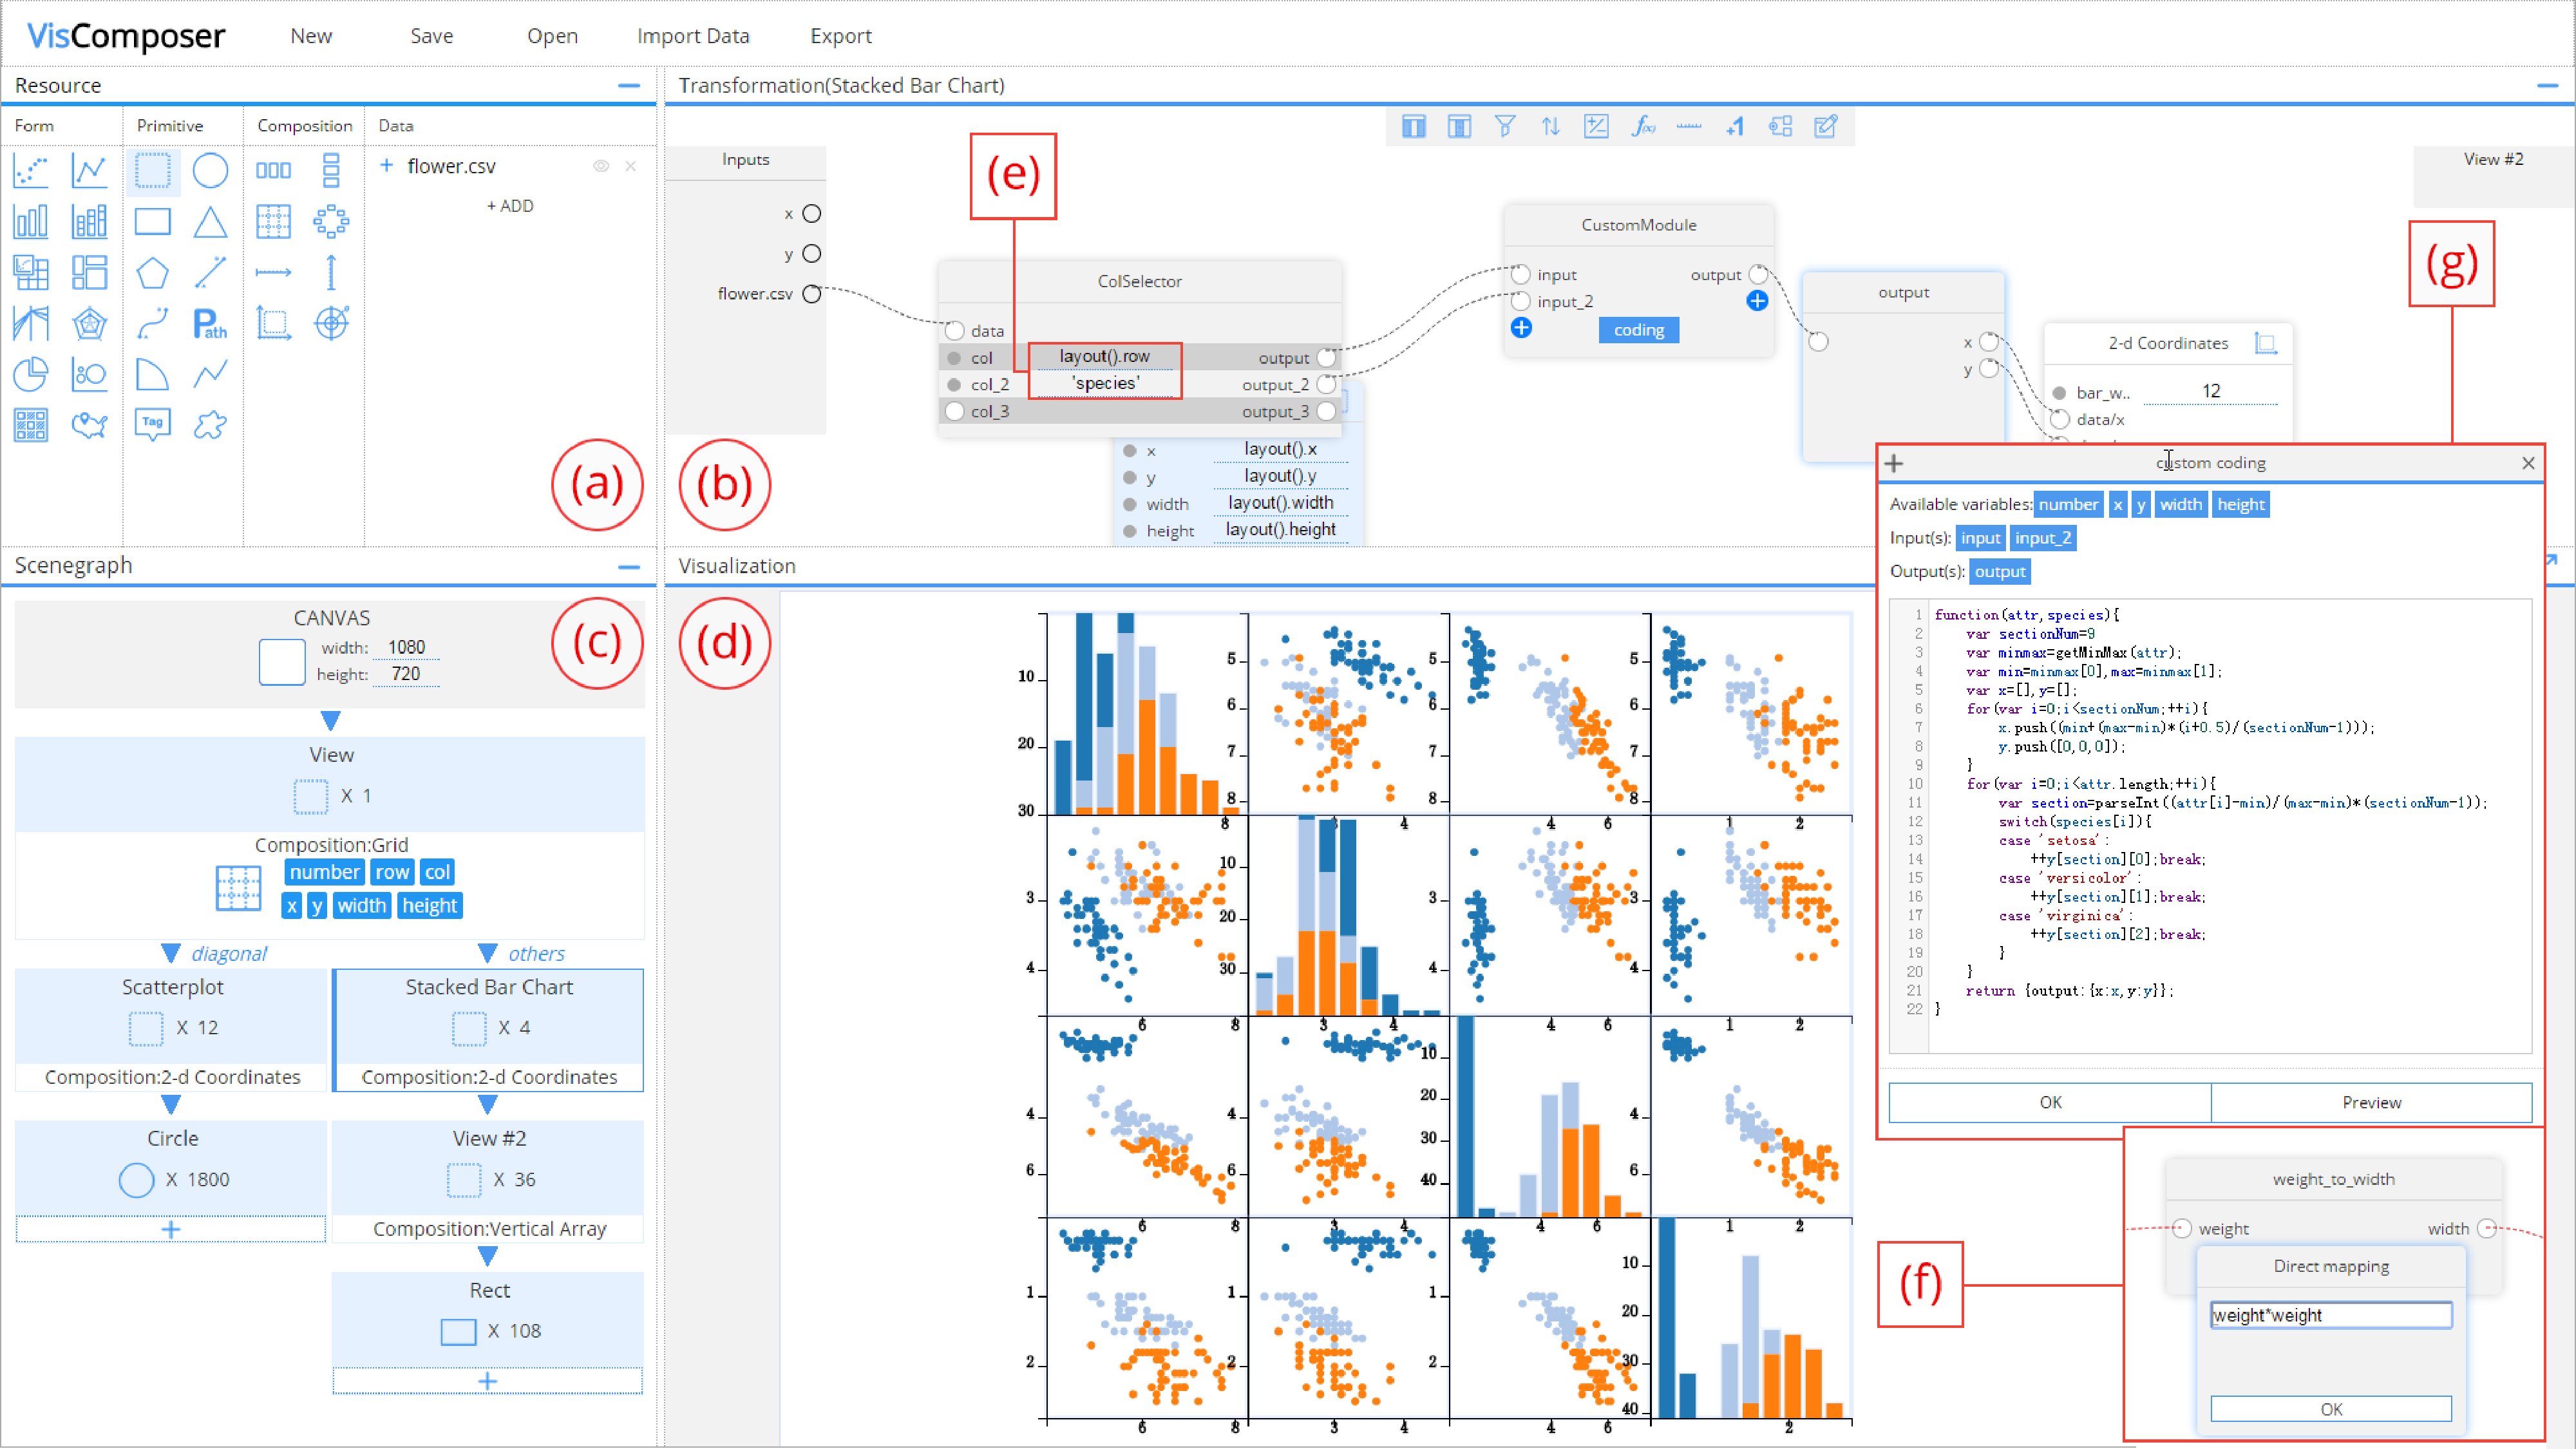
\includegraphics[width=0.98\linewidth]{images/system.pdf}
  \caption{The interface of VisComposer: (a) the resource view, (b) the transformation view, (c) the scenegraph view, and (d) the visualization view. \newline(e) $\scriptsize{\sim}$ (h) Editors for the three types of programmable shaders.
  %and (e) the code editor window of a custom transformation. 
  The scatterplot matrix representation of Iris Flower Dataset is displayed.}
  \label{fg:interface}
\end{figure*}

\subsection{User Interactions}
To compose a visualization, the user can perform operations of the visualization composition model by interactively manipulating data, primitives, composition operators, visual forms, and intermediate structures, such as the scenegraph.  The composition process begins only after a dataset is loaded.  User interactions with the VisComposer interface can be defined as follows.

\noindent \textbf{Selection}: Two types of selection tools are provided to facilitate the specification of points of interest. The lasso selection tool supports brushing a rectangular or an arbitrary shaped region within the visualization or transformation view to select data items or primitives directly. Alternatively, the user can select the data items or primitives by double clicking on the nodes or links in the scenegraph view.

\noindent \textbf{Drag-and-drop}: To transfer selected items in or across different views, the user can drag the object from the original view to the destination.

\noindent \textbf{Painting}: The user can freely draw an axis or other geometry in the visualization canvas in order to directly specify the visual design. The paint tools can help the user quickly specify properties of a new visual structure and refine them if needed. A set of docking points are utilized for the purposes of positioning and designing composition modes.

\noindent \textbf{Programming}: In the transformation view and the scenegraph view most of the elements are programmable. The user can bind data by using a short expression in an input box, or create a functional modifier to assign a custom visual mapping. The user can also trigger a code editor and write scripts in JavaScript. Quick debugging of code is enabled by the interactive output of intermediate results in the visualization view. The user can view the programmed effects by examining individual operations in the visualization view.

\noindent \textbf{Annotations}: The user can identify and analyze the results through free-style annotations. Iconic and textual annotations are supported.

\subsection{Two Design Modes}
VisComposer enables both high-level and low-level control features for use by technical developers as well as purely visual controls to enable visualization design by non-technical artists. Two design modes are provided: design from scratch or template-based design.

\noindent \textbf{Design from scratch:} This mode requires the user to build elements from scratch. Generally, the user follows the flowchart depicted in Figure~\ref{fg:flowchart} to craft a visualization. For modification, the user can flexibly erase, restore, and restart an ongoing composition by means of the interface. Any element can be edited by either programming or pre-defined interactions if necessary.

\noindent \textbf{Template-based design} To simplify the customization of effect and share visualization, a high-level manipulation mode is supported by leveraging the visual forms. By default, a visual form can be formulated based on a template representation. When a template is selected or loaded, the environment automatically instantiates the scenegraph structure. All the components in a template are editable and programmable. In this way, the user can bypass the tedious setup steps and dive straightly into the visualization design process.

\subsection{The Implementation Details}
%The implementation of VisComposer is based on HTML5 with jQuery.

\indent \textbf{Data Format:} VisComposer stores and manipulates data as JavaScript Objects. Data sources, such as CSVs, JSONs, can be loaded and converted to objects. VisComposer provides a flexible data type control to improve data import. Profiles of the input data, such as the data types and dimensions, are kept and can be used in the composition process.
%User-defined data could benefit from it by auto detecting or explicitly declaring.

\noindent \textbf{Drawing:} VisComposer outputs a structured representation of primitives.  Then these primitives are sent to the renderer  in a batch mode. In general, there are two modes for rendering the primitives: creating and displaying SVG nodes which support mouse and keyboard interaction from the browser; drawing in the canvas to generate a static result. To support interactive development, VisComposer utilizes the SVG mode during the visualization composition process. Exporting the result in to HTML5 canvas is also supported when publishing the design.
%and then allows for drawing in the canvas when the design is completed.

\noindent \textbf{Interaction:} VisComposer provides rich user controls which are synchronized among different views. For example, moving an element in the visualization view leads to the changes of its \emph{x} and \emph{y} coordinates in the Transformation view; creating a visual mapping in the transformation view modifies the  scenegraph and the visualization.
%Essentially, the user interaction mode mirrors the code writing mode.
In this way, the user can quickly compose a visualization with user-friendly interactions and obtain real-time feedback in the visualization module.
%customize through scripting.

\noindent \textbf{Serialization:} A visualization is composed of a list of JavaScript objects that are referenced to each other. Similar to iVisdesigner~\cite{Yuan:2014:TVCG}, VisComposer serializes all objects and maintains references to enable external storage, loading and reuse of components. VisComposer assigns a universally unique identifier (UUID) to each object that represents references out of memory. The  object collection of a visualization is processed in depth-first order and objects are stored when they first occur. Specifically, we employ an enhanced serialization scheme that the user can only save part of the pipelines or a sub-tree of the scenegraph into an offline file. Other users can import the file to re-use the component as part of the current design.
%A hashmap using UUIDs as keys is built to guarantee objects are stored as references. When there are more than one reference, the keys can be used to restore the structure. Moreover, an identifier which records the object type is stored and refers to the right constructor to be called while restoring.

\noindent \textbf{Reuse and Export:} VisComposer supports the reuse and exportation of visualizations in three ways: 1) The designed visualization can be exported as a bitmap image or vector graph; 2) The workspace can be exported and saved as a template file for future reuse; 3) The design can be packed with a runtime library,  which can be embedded into an HTML page. 